
\chapter{Related Works}

This Chapter will discuss the origins and inspirations for different components of the final network, as well as other works that use 3D Gaussian Splatting. Relevant sources will be:
\cite{kerbl3Dgaussians}
\cite{zou2023triplane}
\cite{yu2021pointbert}
\cite{yu2021pointr}


I will also mention the similarity to vision transformers such as:
\cite{devlin2019bert}
\cite{yu2021diverse}
\cite{Miao2024}


\chapter{Introduction}
This chapter will explain 3D Gaussians and their ability for novel HD view synthesis at high framerates \cite{kerbl3Dgaussians}
It will also give a preliminary explanation as to why i chose a transformer architecture. \cite{vaswani2023attention}

\section{Motivation}
[An Image showing a hole in an otherwise good Scene]\\
This section will highlight the large interest being shown towards gaussians and will explain how gaussian scenes end up with holes that need to be fixed.

\section{Goals}
This section describes my goal of trying to have an existing gaussian scene be understood by a transformer and then continued. Elaborating on the idea of getting a "good" latent space representation of gaussians.

\section{Challenges}
This section will describe the non structural nature of gaussians and the difficulties of regressing them directly \cite{zou2023triplane}.
It will also show a diagram of the attention layer and it's quadratic memory/computational complexity, describing the need to reduce the sequence length.

\chapter{Network Architecture}
This chapter will start of with a diagram and description of the rough structure of the entire network.

\section{Visual Embedding}
This section will describe the Visual Embedding Net with a more closed up diagram. Both the novel encoder and the decoder (same as used in \cite{zou2023triplane}) will be elaborated on.
There will also be some pictures showing the capabilities of the Visual to encode and decode gaussians while retaining good image quality.

\section{DVAE}
This chapter will introduce the DVAE \cite{rolfe2017discrete} as a way comprehend a local pointcloud and convert it to a token and vice-versa.
\subsection{Sampling/Grouping}
This section will elaborate on the underwhelming performance of the commonly used Furthest-Point + KNN Sampling and will compare and contrast it with Random-Point + KNN Sampling.
\subsection{DGCNN}
This section will explain the DGCNN \cite{wang2019dynamic} and how it enables the DVAE to understand local geometries
\subsection{Discretization}
This section will introduce the vocabulary/codebook and how Gumbel-Softmax \cite{jang2017categorical} is used to discretize the resulting logits before sampling from the vocabulary.
\section{Transformer}
This section will talk about the transformer as a whole.
\subsection{Encoder}
This subsection will describe the self-attention mechanism and the positional encoding used in the encoder-blocks of the transformer.
\subsection{Query Generator}
This subsection will describe the Query generator as a way to turn the memory tokens generated by the encoder into positional information of where the missing content is located.
\subsection{Decoder}
This subsection will describe the cross-attention mechanism used to combine the memory and missing content tokens into useful output tokens.
\chapter{Training}
This chapter will explain the training regime used for the transformer. Describing both methods: 1. Training everything together vs 2. Training every component seperately 
\chapter{Results}
This chapter will look at some results, evaluating them both qualitatively and quantitavely. 
\section{Overall Evaluation}
This subsection will focus on the final results obtained.
\section{Vocabulary Analysis}
This subsection will analyze the different tokens learned by the DVAE.

\chapter{Limitations}
This chapter will highlight the limitations currently present in both the architecture and also results obtained

\chapter{Further Work}
\section{Improvements}
This chapter will somewhat speculate on ways that the architecture could be improved and goals i have in mind for future work on this particular problem
\section{Prospects}
This chapter will talk about the things that would become possible if I can achieve a good latent space representation of Gaussian Scenes (such as style-transfer, etc).






% \subsubsection{Vierte Gliederungsebene}

% Drei Gliederungsebenen sollten für kleine Artikel und Ausarbeitungen genügen. 
% Anderenfalls sollte die Strukturierung nocheinmal überdacht werden.

% \paragraph{Paragraph ist die unterste Ebene} \blindtext

% \section{Tabellen einbinden}

% \begin{table}
% \centering
% \begin{tabular}{|c||lr|}\hline
% 1.1 & 1.2 & 1.3 \\ \hline
% 2.1 & 2.2 & 2.3 \\ \hline \hline
% 3.1 & 3.2 & 3.3 \\ \hline
% \end{tabular}
% \caption{Eine simple Tabelle}\label{tab:simple}
% \end{table}


% Tabellen sollten in einer Table-Umgebung eingefügt und mit einer Caption und einem Label versehen werden.
% Ein einfaches Beispiel zeigt Tabelle \ref{tab:simple}.

% Leider sind Tabellen eines der schwierigeren Kapitel in \LaTeX,
% wenn beispielsweise Zellen zusammengefasst werden.
% Tabelle \ref{tab::komplex} zeigt eine etwas aufwendigere Tabelle.


% \begin{table}
% \centering
% \begin{tabular}{c|c|c|c|c|}	
% 	\multicolumn{2}{c}{}
% 	& \multicolumn{3}{c}{\begin{scriptsize}\textbf{GdO-Typ}\end{scriptsize}}
% 	\\ \hhline{~~---}
% 	\multicolumn{2}{c|}{}
% 	& \textbf{reellwertig}
% 	& \textbf{ganzzahlig}
% 	& \textbf{symbolisch}
% 	\\ \hhline{~|----}
% 	\multirow{4}[3]{*}{\rotatebox{90}{\begin{scriptsize}\textbf{EA-Typ}\end{scriptsize}}}
% 	& \textbf{reellwertig}
% 	& direkt
% 	& Rundung
% 	& ---
% 	\\ \hhline{~|----}
% 	& \textbf{ganzzahlig}
% 	& ---
% 	& direkt
% 	& Index
% 	\\ \hhline{~|----}
% 	& \textbf{Zeichenkette}
% 	& Interpretation
% 	& Interpretation
% 	& direkt
% 	\\ \hhline{~|----}
% \end{tabular}
% \caption{Beispiel für eine komplexere Tabelle}\label{tab::komplex}
% \end{table}

% \section{Bilder/Grafiken einbinden}

% Am besten werden Vektorgrafiken verwendet.
% Diese liegen im Idealfall als PDF vor.
% Aber auch EPS kann z.B. sehr einfach konvertiert werden.

% PDF-Grafiken können unter anderem mit Inkscape \cite{inkscape}, OpenOffice Draw \cite{oodraw} kostenlos bearbeitet und erstellt werden.
% Pixelgrafiken sollten unbedingt vermieden werden. 
% Ihre Auflösung sollte mind. 300dpi betragen.

% \subsection{Einfache Abbildungen}

% \begin{figure}
% \centering % zentriert alles in der Figure
% 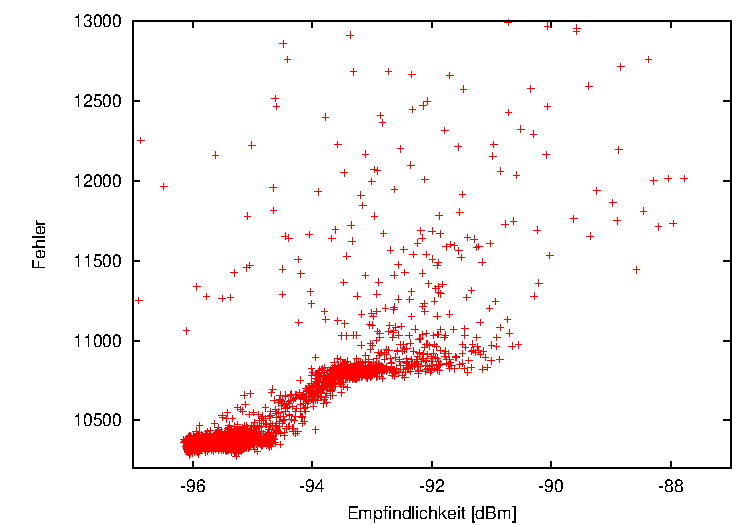
\includegraphics[width=0.6\linewidth]{Images/Chapter/bspgrafik1} % externe Grafik laden
% \caption{Dieses Diagramm ist ein Beispiel für eine einfache Abbildung.}\label{fig:testabb}
% \end{figure}


% Eine Abbildung sollte sich immer in einer Figure-Umgebung befinden.
% In dieser kann sie mit einer Caption beschrieben werden
% und sie kann über ein Label gekennzeichnet werden (vgl. Abbildung \ref{fig:testabb}).

% Dabei muss es keine Grafik sein, die in eine Figure-Umgebung geladen wird.
% Es kann dort ganz normal \LaTeX geschrieben werden,
% wie Abbildung \ref{fig:testabb2} zeigt.

% \begin{figure}
% \centering
% \fbox{\parbox{0.9\linewidth}{\centering In einer Figure muss keine Grafik stehen... Eine Abbildung kann im Prinzip alles sein.}}
% \caption{Dies ist eine Bildunterschrift} \label{fig:testabb2}
% \end{figure}

% \subsection{Unterabbildungen}

% \begin{figure}%
%   \centering
%    \subfloat[Die erste Unterabbildung]{\label{fig:subfig1}%
%        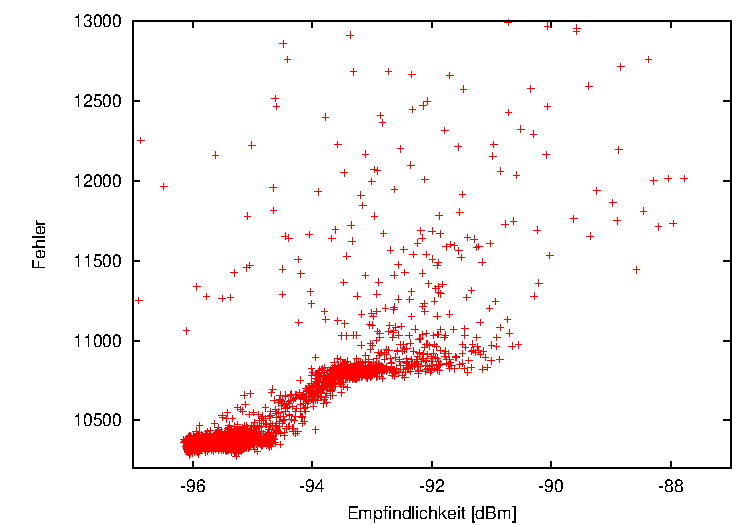
\includegraphics[width=0.48\linewidth]{Images/Chapter/bspgrafik1}
%    }\hfill
%    \subfloat[Die zweite Unterabbildung]{\label{fig:subfig2}%
%        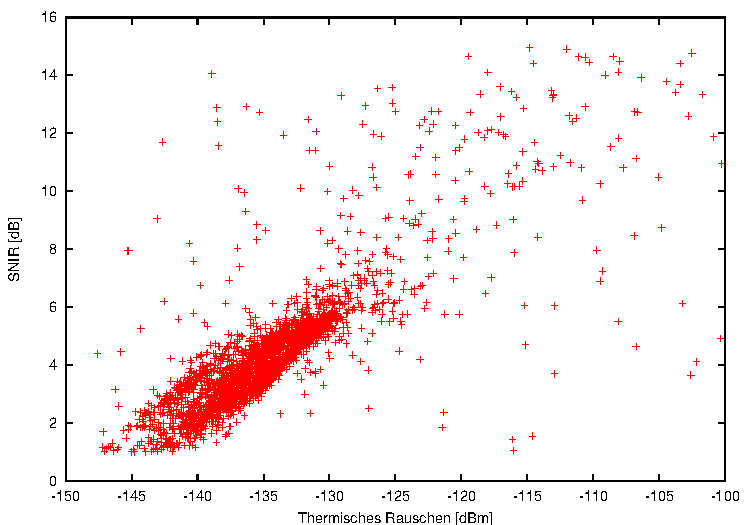
\includegraphics[width=0.48\linewidth]{Images/Chapter/bspgrafik2}
%    }
%    \caption{Beispiel für Unterabbildungen}
%    \label{fig:subfigexample}
% \end{figure}


% In manchen Fällen ist es sinnvoll eine Abbildung in Unterabbildungen zu teilen.
% In Abbildung \ref{fig:subfigexample} wird dies gezeigt.
% Die Abbildungen \ref{fig:subfig1} und \ref{fig:subfig2} sind Unterabbildungen.

% \section{Formeln}

% Für seinen Formelsatz ist \LaTeX besonders bekannt, weshalb es hier nicht an einem kleinen Beispiel (vgl. Formel \ref{eq::gewichtsumme}) fehlen soll.

% \begin{equation}
% f\idx{sim}(g,U)=\sum\limits^{n\idx{M}}_{\mu=1} w_\mu\cdot c_i( M_\mu(g,U)) \label{eq::gewichtsumme}
% \end{equation}

% \section{Quelltexte einbinden}

% \begin{figure}[t]
% \begin{lstlisting}[language=java, caption={Beispiel für ein Listing},  label=lst:bsplst]
% public class RadioFitness extends BasicFitness {
%   ...
%   SimResultReader result = new SimResultReader();
%   ...
%   protected void readResult(Scenario s) throws FitnessException {
%     result.readFrom(s.getExecEnv().getExecutionDir());
%   }

%   protected double getRawMetric(String name) throws FitnessException {
%     if(name.equals("delivery rate")
%       return result.getNumSendData()/result.getNumReceivedData();
%     else if(name.equals("latency"))
%       return results.getLatency();
%     else ...
%   } // comment
%   ...
% }
% \end{lstlisting}
% \end{figure}


% Ein Beispiel für ein Java-Listing zeigt Listing \ref{lst:bsplst}.


% \section{Zitieren von Quellen}

% Aussagen wollen gut belegt sein.
% Hier sind willkürlich \cite{FejF08} beispielhafte Zitierungen \cite{Deming1986} angegeben,
% die keinen inhaltlichen Bezug zu diesem Text aufweisen.
% Vielmehr geht es darum beispielhaft zu zitieren.
% Es können auch mehrere Quellen angegeben werden \cite{biturl,Rost2009} (auch hier wieder ohne inhaltlichen Bezug).

% Die Literaturangaben werden in einer Datenbank verwaltet,
% die in einer .bib-Datei gespeichert wird.
% In dieser kann auch nicht zitierte Literatur stehen.
% Eine gute Software zur Bearbeitung dieser Datenbank ist JabRef \cite{jabref}.